\chapter{The Large Hadron Collider}
The primary reference for this chapter was \cite{LHC} and it should be consulted for further reading.

Constructed by the European Centre for Nuclear Research (CERN), the Large Hadron Collider (LHC) \cite{LHC} is the world's largest particle accelerator. It has provided some of the experimental confirmation of the Standard Model. Located underground and crossing the Franco-Swiss border at four points (most of the tunnel is located in France), the LHC was installed in the existing 26.7 km tunnel that was previously used by the Large Electron-Positron Collider (LEP). Initially approved by the CERN Council in 1994, construction of the LHC received substantial contributions from CERN member-states and non-member states alike. CERN was chosen as the location due to the advantage of being able to use the pre-existing LEP tunnel. Because the LHC is a particle-particle collider (as opposed to a particle-antiparticle collider), it is composed of two rings with counter-rotating beams.\footnote{Particle-antiparticle colliders can have both beams within the same ring \cite{LHC}.} Each of the two beam pipes is kept at ultrahigh vacuum $10^{-10}$ Torr \cite{vacuum} in order to reduce the possibility of undesirable collisions with gas molecules.

The construction of the LHC was primarily approved in order to discover beyond the Standard Model physics. It has two high luminousity\footnote{Both originally aiming for a peak luminousity of $\mathcal{L} = 10^{34}$cm$^{-2}$s$^{-1}$.} experiments: ATLAS (A Toroidal LHC ApparatuS) \cite{ATLAS} and CMS (Compact Muon Solenoid) \cite{CMS}, as well as two low luminousity experiments: LHCb (Large Hadron Collider bottom)\footnote{Originally aiming for a peak luminousity of $\mathcal{L} = 10^{32}$cm$^{-2}$s$^{-1}$.} \cite{LHCb} which is primarily concerned with the physics of b-quarks, and TOTEM (TOTal Elastic and diffractive cross section Measurement)\footnote{Originally aiming for a peak luminousity of $\mathcal{L} = 2 \times 10^{29}$cm$^{-2}$s$^{-1}$.} \cite{TOTEM} which specialises in the detection of small-angle elastic proton scattering.  The LHC is versatile and can also be operated to collide heavy-ions instead of protons. ALICE (A Large Ion Collider Experiment)\footnote{Originally aiming for a peak luminousity of $\mathcal{L} = 10^{27}$cm$^{-2}$s$^{-1}$.} \cite{ALICE} is dedicated to the detection and analysis of these heavy-ion collisions.

As with all particle accelerators, the protons are steered by means of powerful magnetic fields. Colliding the counter-rotating beams of protons requires opposite magnetic fields in both of the LHC rings. However, there is not enough physical space for two separate rings of magnets in the LHC tunnel. In order to compensate for this, the LHC uses twin bore magnets that consist of two sets of coils and beam channels within the same mechanical structure and cryostat. The magnetic system itself consists of 1232 dipole magnets, each with a length of 15 metres, which are concerned with bending the proton beams, and 392 quadrupole magnets of lengths varying between five and seven metres which are concerned with focusing the beam. This magnet system produces fields above 8 T and is kept at a temperature of 2 K by approximately 96 tonnes of superfluid helium-4, making the LHC the world's largest cryogenic facility \cite{cryo}.

The LHC is fed with protons by means of the injector chain: a series of accelerators that successively increase the energy of the protons. The accelerators that make up the injector chain were previously existing accelerators at CERN which were repurposed and upgraded in order to provide the LHC with protons. In order of increasing energy the constituents of the injector chain are: \emph{Linac2}, \emph{Proton Synchrotron Booster} (PSB), \emph{Proton Synchrotron} (PS), and ultimately the \emph{Super Proton Synchrotron} (SPS) which then supplies protons for use by the LHC. The injector chain is illustrated in figure \ref{lhc_injectors_image}.

\begin{figure}
\centering
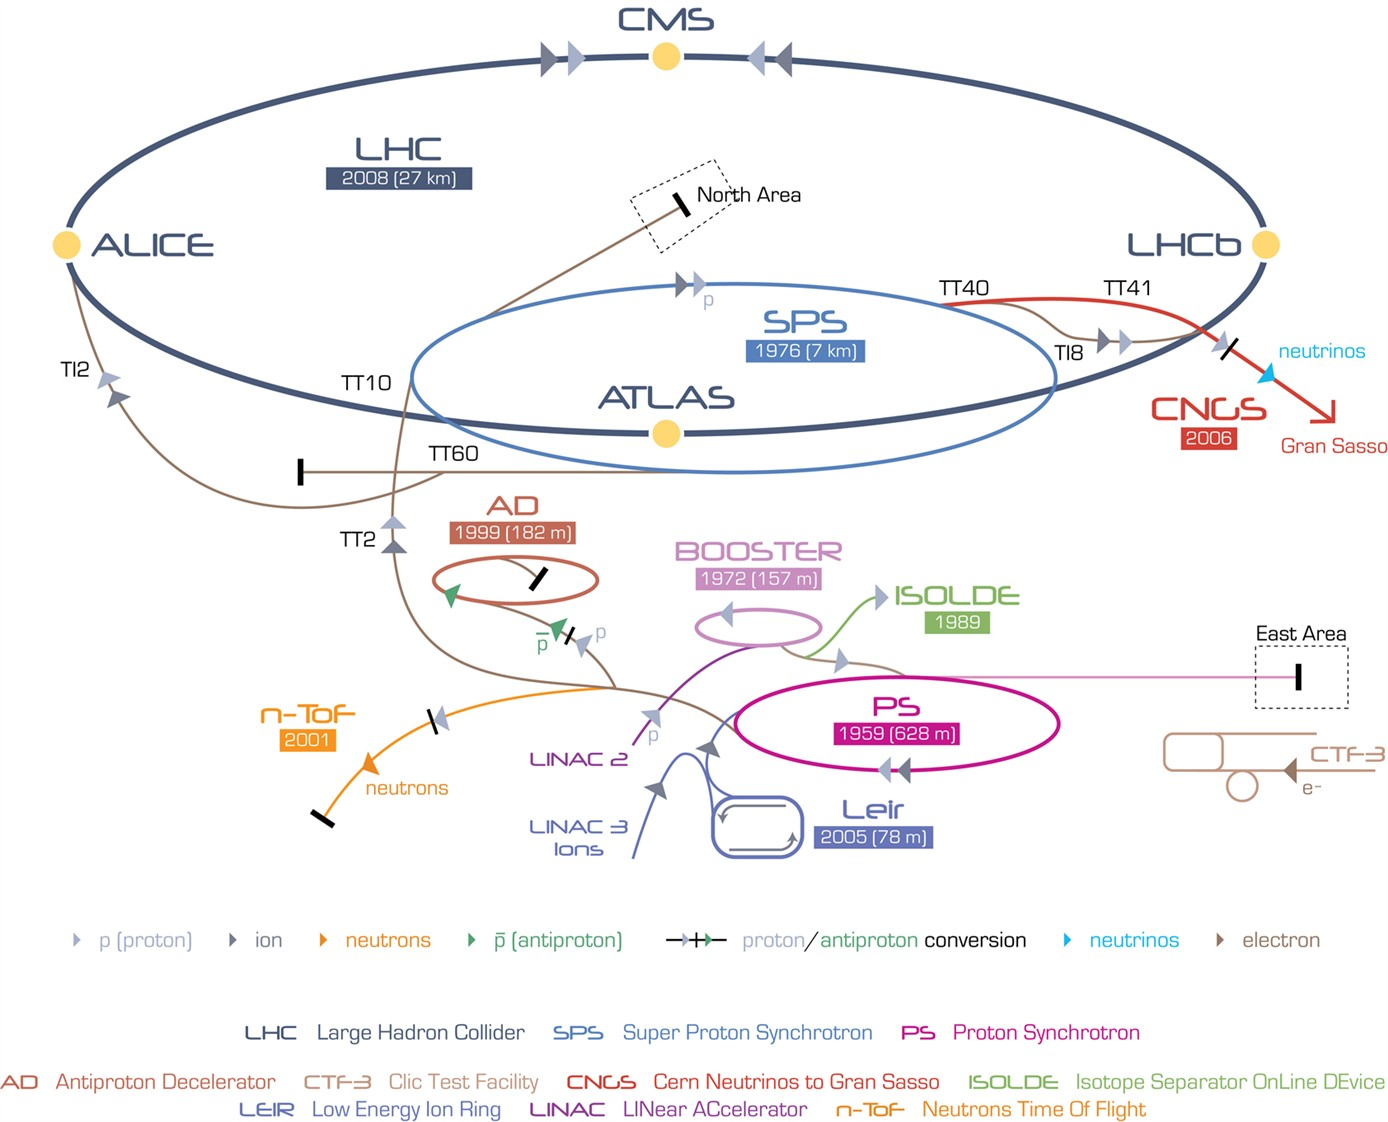
\includegraphics[width=.93\textwidth]{images/lhc_injectors.png}
\caption{Illustration of the LHC's injector chain. \cite{lhc_injector_image}}
\label{lhc_injectors_image}
\end{figure}